\documentclass[12pt]{beamer}

\mode<presentation> {
	
	
	%\usetheme{Madrid}
	%\usepackage{times}
	\renewcommand{\familydefault}{\rmdefault}
	\usetheme{CambridgeUS}
	\usepackage[latin1]{inputenc}
	\usefonttheme{professionalfonts}
	\usepackage{times}
	\usepackage{tikz}
	\usepackage{amsmath}
	\usepackage{verbatim}
	\usepackage{enumerate}
	\usepackage{setspace}
	\usetikzlibrary{arrows,shapes}
	\usepackage{amsmath}
	\usepackage{eurosym}
	\usepackage{framed}
	\usepackage{extarrows}
}

\usepackage{graphicx}
\usepackage{booktabs}
\usepackage{url}
%----------------------------------------------------------------------------------------
%	TITLE PAGE
%----------------------------------------------------------------------------------------


\title{SFM01-VaR-blockmaxima-backtesting}

\author[]{Liang chen 15620151152901\\Du yao 15620151152897\\Feng xiaowei 15520151152644\\Zi xuefei 15620151152919} % Your name
\institute[]{
	\textsl{July 13th,2016}
}
\date[July 13$^{th}, 2016$]{} % Date, can be changed to a custom date


\begin{document}
	
\begin{frame}
	\titlepage
\end{frame}


\section{Data}
\begin{frame}
	\frametitle{Data}
	\begin{itemize}
		\item Data source: $http://en.boerse-frankfurt.de$.
		\item Data range: all the trading days from $2002-01-01$ to $2016-06-30$, daily data.
		\item Data files:$Bayer-close-0216.txt$, $Bmw-close-0216.txt$, $Siemens-close-0216.txt$.
	\end{itemize}
\end{frame}


\section{Steps of procedure}
\begin{frame}
	\frametitle{Steps of procedure}
		1.Construct a portfolio: $V=Bayer+Bmw+Siemens$
\end{frame}


\section{Steps of procedure}

\begin{frame}
	\frametitle{Steps of procedure}
        2.Calculate the $VaR$ of the portfolio by using Block Maxima Model.
	\begin{itemize}
		\item Decompose negative returns $\{X_t\}_{t=1}^T$ into $k$ non-overlapping sets.
		\item Define $\{Z_j\}_{j=1}^k$ where $Z_j=max\{X_{(j-1)n+1},...,X_{jn}\}$.
		\item For $\{Z_j\}_{j=1}^k$, fit generalized extreme value distribution $G_{\gamma}(\frac{x-\mu}{\sigma})$.
        \item $VaR$ at $\alpha$: $VaR(\alpha)=\mu+\frac{\sigma}{\gamma}[(-log(1-\alpha^n))^{-\gamma}-1]$.
        \item T denotes the number of observations.
	\end{itemize}
\end{frame}


\section{Steps of procedure}

\begin{frame}
	\frametitle{Steps of procedure}
        3.Backtesting with Moving Window Method.
	\begin{itemize}
		\item Daily P\&L of the portfolio from $2002-01-01$ to $2016-06-30$.
        \item Static windows of size $h=250$ scrolling in time $t$ for $VaR$ estimation $\{X_t\}_{t=s-h+1}^{s}$ for $s=h,...,T$.
        \item Moving window results: Estimates of the parameters of $G_{\gamma}(\frac{x-\mu}{\sigma})$ by MLE, that is, $\{\hat{\mu}_t\}_{t=h}^T$, $\{\hat{\sigma}_t\}_{t=h}^T$, $\{\hat{\gamma}_t\}_{t=h}^T$, and $\{\widehat{VaR}_{1-\alpha}^t\}_{t=h}^T$.
        \item Take the opposites of $\{\widehat{VaR}_{1-\alpha}^t\}_{t=h}^T$ and find the outliers.
	\end{itemize}
\end{frame}



\section{Steps of procedure}
\begin{frame}
	\frametitle{Steps of procedure}
        4.Calculate exceedances ratio
	\begin{itemize}
        \item $\hat{\alpha}=\frac{1}{T-h}\sum_{t=h+1}^{T}I\{X_t<-\widehat{VaR}_{1-\alpha}^{t}\}$
	\end{itemize}
\end{frame}


\section{Steps of procedure}
\begin{frame}
	\frametitle{Steps of procedure}
        5.Realizations by R and Matlab.
	\begin{itemize}
		\item Value-at-Risk estimation at $\alpha = 0.05$ level for portfolio, with size of moving window $h=250$ and size of block $n = 16$.
        \item Backtesting result with R: $\hat{\alpha}= 0.0495$.
        \item Backtesting result with Matlab: $\hat{\alpha}= 0.0501$.
        \item The difference is caused by the different estimation procedure of GEV in the two softwares.
	\end{itemize}
\end{frame}


\section{Steps of procedure}
\begin{frame}
	\frametitle{Steps of procedure}
	\begin{figure}[htpb!]
      \centering
      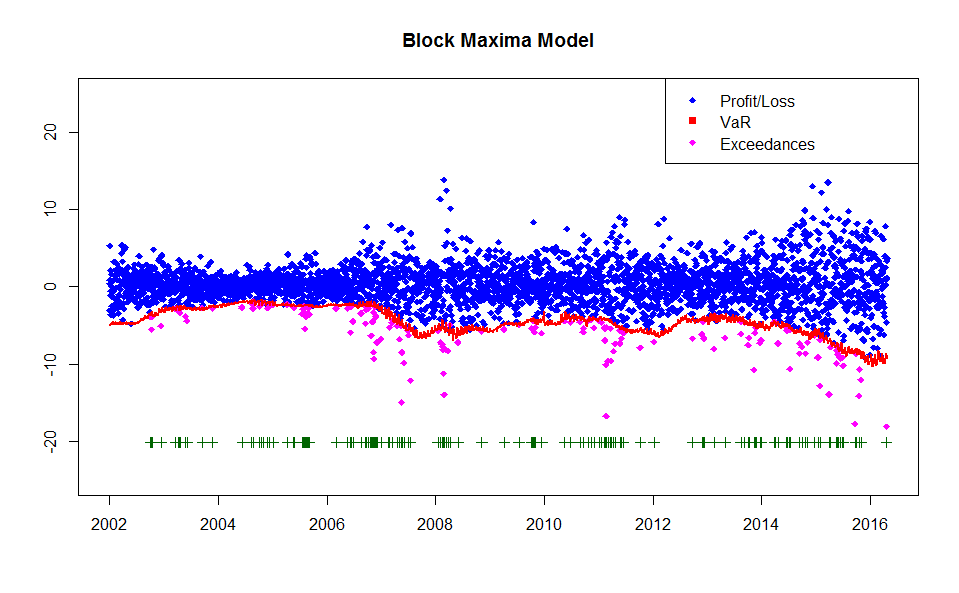
\includegraphics[width=9cm,height=6cm]{VaR_BBM_backtesting_R.png}
      \caption{$VaR-BBM-backtesting-R$}
    \end{figure}
\end{frame}


\section{Steps of procedure}
\begin{frame}
	\frametitle{Steps of procedure}
      \begin{figure}[htpb!]
        \centering
        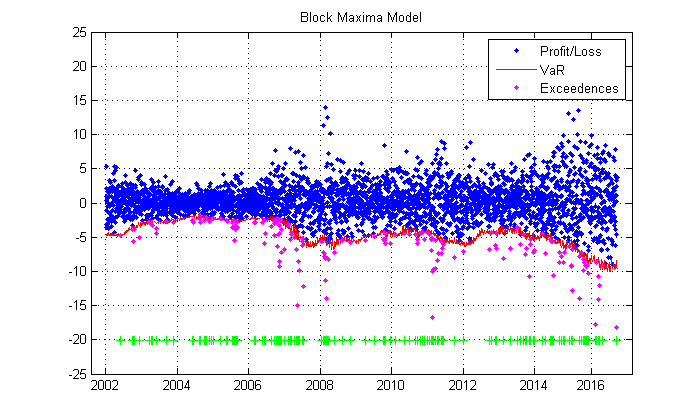
\includegraphics[width=9cm,height=6cm]{VaR_BBM_backtesting_Matlab.png}
        \caption{$VaR-BBM-backtesting-Matlab$}
      \end{figure}
\end{frame}


\end{document}
